\documentclass[border=6pt]{standalone}
\usepackage{tikz}
\usetikzlibrary{arrows.meta,calc}
\begin{document}
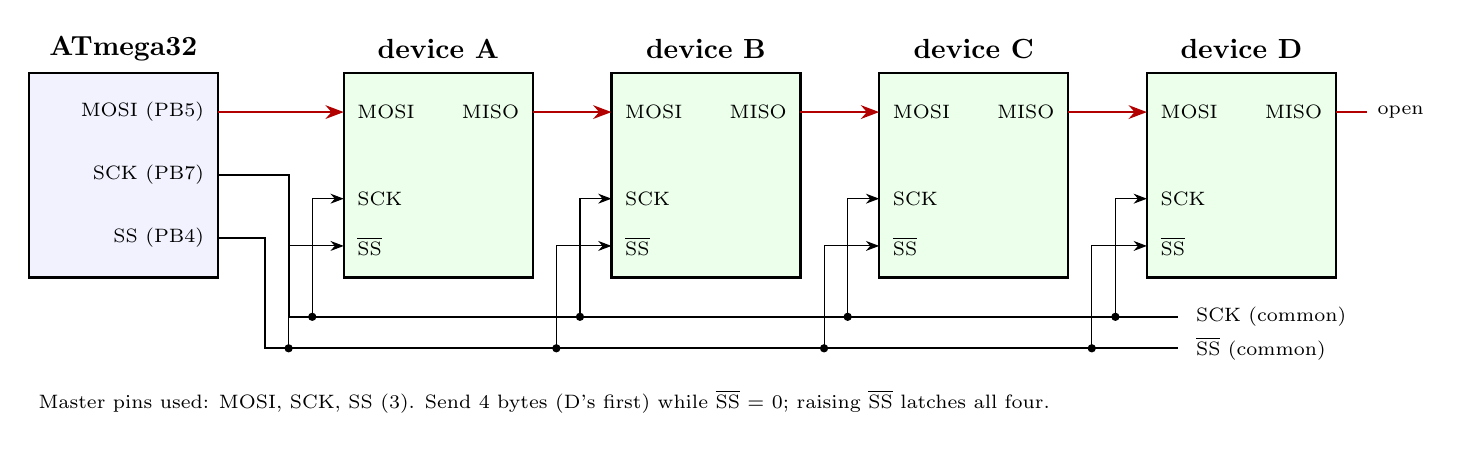
\begin{tikzpicture}[>=Stealth,font=\small]
% master
\draw[thick,fill=blue!5] (0,0) rectangle (2.4,-2.6);
\node[font=\bfseries] at (1.2,0.3) {ATmega32};
\foreach \y/\t in {-0.5/MOSI (PB5),-1.3/SCK (PB7),-2.1/SS (PB4)} \node[font=\scriptsize,anchor=east] at (2.35,\y) {\t};
% devices A-D
\foreach \i/\n in {0/A,1/B,2/C,3/D} {
  \pgfmathsetmacro{\x}{4.0+3.4*\i}
  \draw[thick,fill=green!8] (\x,0) rectangle (\x+2.4,-2.6);
  \node[font=\bfseries] at (\x+1.2,0.3) {device \n};
  \node[font=\scriptsize,anchor=west] at (\x+0.05,-0.5) {MOSI};
  \node[font=\scriptsize,anchor=east] at (\x+2.35,-0.5) {MISO};
  \node[font=\scriptsize,anchor=west] at (\x+0.05,-1.6) {SCK};
  \node[font=\scriptsize,anchor=west] at (\x+0.05,-2.2) {$\overline{\mathrm{SS}}$};
}
% data chain
\draw[->,thick,red!70!black] (2.4,-0.5) -- (4.0,-0.5);
\draw[->,thick,red!70!black] (6.4,-0.5) -- (7.4,-0.5);
\draw[->,thick,red!70!black] (9.8,-0.5) -- (10.8,-0.5);
\draw[->,thick,red!70!black] (13.2,-0.5) -- (14.2,-0.5);
\draw[thick,red!70!black] (16.6,-0.5) -- (17.0,-0.5) node[right,font=\scriptsize,black]{open};
% SCK and SS buses
\draw[thick] (2.4,-1.3) -- (3.3,-1.3) -- (3.3,-3.1) -- (14.6,-3.1);
\draw[thick] (2.4,-2.1) -- (3.0,-2.1) -- (3.0,-3.5) -- (14.6,-3.5);
\foreach \i in {0,1,2,3} {
  \pgfmathsetmacro{\x}{4.0+3.4*\i}
  \draw[->] (\x-0.4,-3.1) |- (\x,-1.6);
  \fill (\x-0.4,-3.1) circle (1.5pt);
  \draw[->] (\x-0.7,-3.5) |- (\x,-2.2);
  \fill (\x-0.7,-3.5) circle (1.5pt);
}
\node[font=\scriptsize,anchor=west] at (14.7,-3.1) {SCK (common)};
\node[font=\scriptsize,anchor=west] at (14.7,-3.5) {$\overline{\mathrm{SS}}$ (common)};
\node[font=\scriptsize,align=left,anchor=north west] at (0,-3.9) {Master pins used: MOSI, SCK, SS (3). Send 4 bytes (D's first) while $\overline{\mathrm{SS}}$ = 0; raising $\overline{\mathrm{SS}}$ latches all four.};
\end{tikzpicture}
\end{document}
